\documentclass{article}


% arxiv style file, see https://github.com/kourgeorge/arxiv-style
\usepackage{arxiv}

\usepackage[utf8]{inputenc} % allow utf-8 input
\usepackage[T1]{fontenc}    % use 8-bit T1 fonts
\usepackage{hyperref}       % hyperlinks
\usepackage{url}            % simple URL typesetting
\usepackage{booktabs}       % professional-quality tables
\usepackage{amsfonts}       % blackboard math symbols
\usepackage{nicefrac}       % compact symbols for 1/2, etc.
\usepackage{microtype}      % microtypography
\usepackage{lipsum}		% Can be removed after putting your text content
\usepackage{graphicx}
\usepackage{natbib}
\usepackage{doi}

\usepackage{mathtools}

\graphicspath{ {./figures/} }

\title{A template for the \emph{arxiv} style}

%\date{September 9, 1985}	% Here you can change the date presented in the paper title
%\date{} 					% Or removing it

\author{ \href{https://orcid.org/0000-0003-4058-1543}{
\includegraphics[scale=0.06]{orcid.pdf}\hspace{1mm}Malte~Schierholz}\thanks{This work has been created during a research stay at the Machine Learning for Public Policy lab at Carnegie Mellon University} \\
	Department of Statistics\\
	Ludwig-Maximilians-Universität München\\
	80539 Munich \\
	\texttt{hippo@cs.cranberry-lemon.edu} \\
	%% examples of more authors
	%% \AND
	%% Coauthor \\
	%% Affiliation \\
	%% Address \\
	%% \texttt{email} \\
	%% \And
	%% Coauthor \\
	%% Affiliation \\
	%% Address \\
	%% \texttt{email} \\
	%% \And
	%% Coauthor \\
	%% Affiliation \\
	%% Address \\
	%% \texttt{email} \\
}

% Uncomment to remove the date
%\date{}

% Uncomment to override  the `A preprint' in the header
%\renewcommand{\headeright}{Technical Report}
%\renewcommand{\undertitle}{Technical Report}
\renewcommand{\shorttitle}{\textit{arXiv} Template}

%%% Add PDF metadata to help others organize their library
%%% Once the PDF is generated, you can check the metadata with
%%% $ pdfinfo template.pdf
\hypersetup{
pdftitle={A template for the arxiv style},
pdfsubject={q-bio.NC, q-bio.QM},
pdfauthor={David S.~Hippocampus, Elias D.~Striatum},
pdfkeywords={First keyword, Second keyword, More},
}

\begin{document}
\maketitle

\begin{abstract}
	\lipsum[1]
\end{abstract}


% keywords can be removed
\keywords{First keyword \and Second keyword \and More}


\section{Introduction}\label{sec:introduction}

Time is a crucial factor in many data sets, but best practices of how date variables should be used in analyses do not exist.

For example, consider the donorsChoose data set.\footnote{The KDD Cup 2014 DonorsChoose dataset is available from \href{https://www.kaggle.com/c/kdd-cup-2014-predicting-excitement-at-donors-choose/data}{Kaggle}. The \href{https://github.com/dssg/donors-choose}{Data Science for Social Good Github Repository} lays out a possible route of analysis, our reference method here.} DonorsChoose (\url{https://www.donorschoose.org/}) allows teachers to crowdsource funding for various projects, like buying a microwave that lets them cook with children in preschool. The requested items are shipped only when enough citizen donors support the project, and funding goals are met within four months. As data scientists, we want to identify postings automatically that are at risk of not meeting its funding goal, and before they get published, with the intention to help teachers improve their postings and, thereby, their chance to get funded. Several projects are posted each day. It is not unlikely that factors affecting the success of funding change over time.

A common framework to predict outcomes in settings like DonorsChoose is implemented in triage\footnote{\url{https://pypi.org/project/triage/}}, a python package. The framework is as follows: 
\begin{itemize}
    \item \textit{Training data}: Pool all observations from a given month (or any other user-defined interval), forming the training data. Outcomes are observed up to four months after (in the DonorsChoose setting, but in general depending on the task at hand).
    \item \textit{Model training}: Employ any statistical learning technique (e.g., random forest, boosting, linear regression, ...) to generate a predictive model.
    \item \textit{Deployment/Test data}: The predictive model gets deployed on future time periods. It is good practice to evaluate it first. For evaluation, all observations from the month after training outcomes become available (or another interval duration) are pooled, forming the test data.
    \item \textit{Check sensitivity}: Repeat the steps above for different training/test months (or other interval duration), while keeping the time period between both data sets constant.
\end{itemize}
But what are the optimal intervals for pooling the training/test data when the dynamics shift over time? How much shift is to be expected happening after training and before the model can get deployed? Statistical learning theory provides little guidance here, since a standard theoretical assumption---training and test data are drawn from the same probability distribution---is not met. Instead, the distribution $p_t(y, x)$ might shift over time and in the most extreme case, if there were a sudden shock between training and testing, extrapolation from training to the deployment period would be impossible. The contrary case, that the distribution $p_t(y, x)$ is constant in time, is the implicit working assumption in the above framework, but real data rarely behave this way (as one easily sees with the sensitivity checks). The middle ground is most realistic, namely that $p_t(y, x)$ is continuous in time. While researchers have proposed various ways to correct for distribution shift \citep[e.g.,][p. 133ff.]{varshney_trustworthy_2021}, we are not aware of any research that aims to model the size of such shifts, while assuming continuity.

In our approach, we do not pool training data, but model changing parameters at consecutive time points, adopting techniques from the state space literature. This is advantageous for three reasons. First, we can generate credibility intervals describing the uncertainty when predicting future outcomes. Second, our approach automatically detects possible long-term trends that would easily be missed within the standard framework mentioned above. Third, shocks that occur during the training period in the standard framework can have dramatic consequences for model performance (using training data from before the shock bodes ill for extrapolation into the future), but our approach would deploy parameters that were estimated at the end of the training periods, only representing the most recent dynamics after the shock ended.

This paper proceeds as follows. ...

\section{Model}\label{sec:model}

Take a data set with $i = 1, ..., N$ observations. We want to predict an outcome $y$ given predictors $x$. $y$ will be continuous in the beginning, but we will also test binary outcomes in later simulations. While this situation can be modeled by least-squares regression (or any other regression algorithm), our situation differs because we have information about time: The predictors about a given individual are available at some time point $t \in \{1, ..., T\}$. The outcome will be observed later within a fixed time span (if it were already known, we would not need to predict it).

Let $y_{i(t)}$ be the outcome of individual $i$, observed within a fixed period after $t$ (not yet available at time $t$, although the notation suggests so!). $x_{i(t)p}$ are the $p = 1, ..., P$ predictors that were available at the time of prediction $t$. (The subscript $t$ indicates that we make predictions at different times, not the time of observation.) $\beta$, $\alpha$ and $\nu$ are parameter matrices, each of dimension $T*P$, with entries for each predictor at all time points.

Our modeling approach is described by the following equations:
\begin{eqnarray}
y_{i(t)} | x_{i(t)p} \sim N(\sum_p x_{i(t)p} \beta_{tp}, \sigma_y^2) \textrm{~~~~~~~~~~~~~~~} & \textrm{(observation equation)} \\
\beta_{tp} \sim N(\alpha_{tp}, \sigma^2_{\beta})\textrm{~~~~~~~~~~~~~~~~~~~~~~~~~~~~~~} & \textrm{(fluctuation equation)} \\
\alpha_{t+1,p} \sim N(\alpha_{t,p} + \nu_{t,p}, \sigma^2_{\alpha})\textrm{~~~~~~~~~~~~~~~~~~} & \textrm{(state equation)} \\
\nu_{t+1,p} \sim N(\nu_{t,p}, \sigma^2_{\eta})\textrm{~~~~~~~~~~~~~~~~~~~~~~~~~~~~~~} & \textrm{(trend equation, optional)}
\end{eqnarray}

Without prior knowledge, we use non-informative priors for the variances $\sigma_y^2$, $\sigma^2_{\beta}$, $\sigma^2_{\alpha}, \sigma^2_{\eta}$ and for the vectors $\alpha_{1,p}$ and $\nu_{1,p}$ at $t=1$.

The observation equation would be a least-squares regression if it were not for the subscript $t$, indicating that parameters $\beta$ vary and depend on the hour/day/year (application-specific) of prediction. There may be very few observations at each time point, impeding the estimation of $\beta$. Since state-space models (also known as dynamic linear models) \citep{prado_time_2010, shumway_time_2011, durbin_time_2012} were developed for situations, in which a single observation (or none) is available at each $t$, they appear well-suited for our analysis. The state equation and the trend equation are well-known concepts in that literature, and many extensions are available from it.

Unlike other approaches we are aware of, we include a fluctuation equation (in state-space terminology this would be called observation equation), only possible because we usually have (far) more than one observation at each time point. The implication is this: If we had at each time point an infinite number of observations, $\sigma^2_\beta$ would go to $\infty$ and the $\beta_t$ would be equal to estimates of $t$ independent logistic regressions. If there are, conversely, just very few observations at each time point, $\sigma^2_\beta$ will turn out to be small and observations from neighboring time points weigh in strongly in the estimation of $\beta_t$.

We carry out a Bayesian approach and estimate the model using the probabilistic modeling language Stan \citep{stan_development_team_rstan_2021}, see supplementary files.

\section{Simulation Study for Continuous Outcomes}

To test the estimation procedure, we do a simulation study. We start with a time series $ts_t$ containing 100 time points, shown in red in Figure \ref{fig:fig1} (the Nile data from \citep{durbin_time_2012}. Our simulated will have 5 observations at each time point. The covariates $x_{i1} \sim N(0,1)$ and $x_{i2} \sim N(0, 20)$ are drawn from two separate normal distributions. The observed $y$-values (the black dots in Figure \ref{fig:fig1}) are then generated using the formula

\begin{align}
y_{i(t)} = ts_t + 30 \cdot x_{i1} + 0 \cdot x_{i2} + N(0, 5)    
\end{align}

The goal of the simulation is to see whether we can recover the original time series and the parameters $\beta_{1t} = 30$ and $\beta_{2t} = 0$ using observed data $x_{i(t)1}$, $x_{i(t)2}$ and $y_{i(t)}$ only. Only observations from $t = 1, ..., 70$ are used for model training, the final 30 time points are used for evaluation.

\begin{figure}
	\centering
	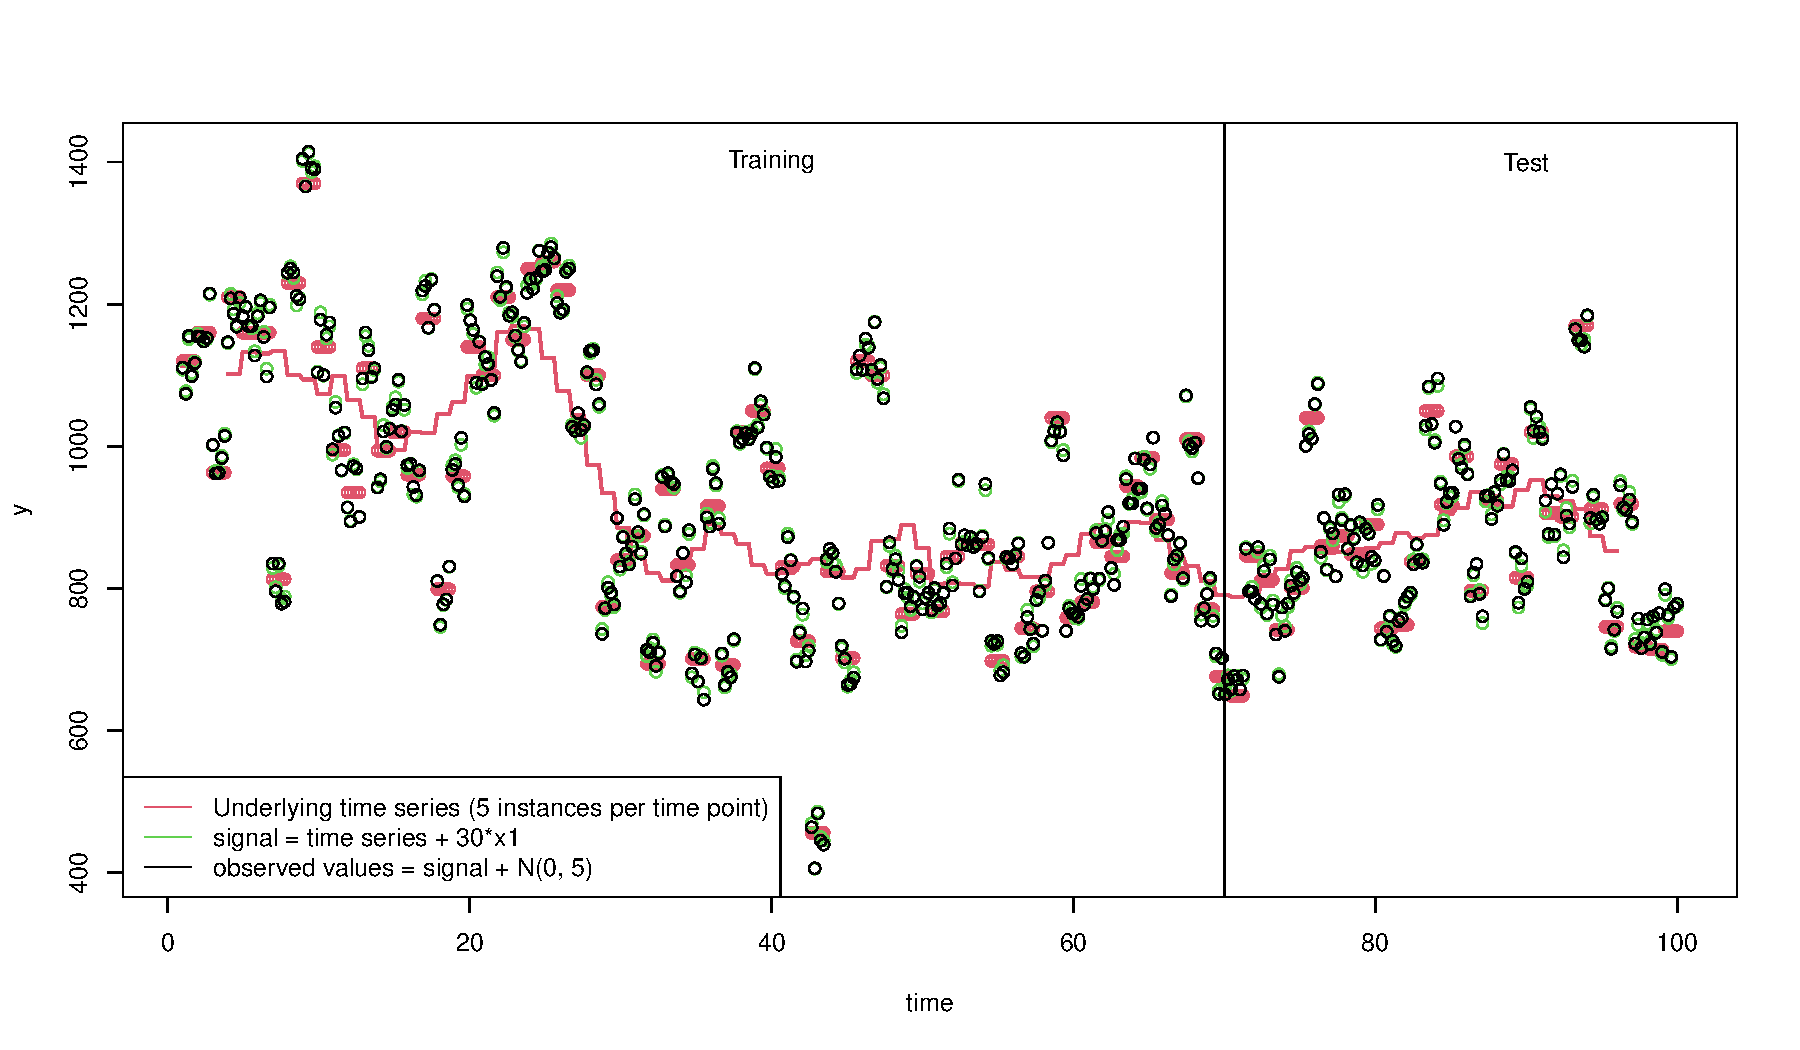
\includegraphics[width=630pt, angle=270]{visualize_simulated_data.pdf}
	\caption{Overview of simulated data.}
	\label{fig:fig1}
\end{figure}

Figure \ref{fig:fig2} shows the smoothed time series from our model (in black) against the original time series $ts_t$ (in red). During the training phase, the smoothed time series closely aligns to the moving average, showing that the model is capable to detect changes over time. This time series exhibits strong changes over time, and for this reason it is hard make predictions of how the series will behave during the test period, as evidence by the widening credibility intervals.

Figure \ref{fig:fig3} shows the estimated parameters for $\beta_{1t}$ and $\beta_{2t}$. The true values (know from the simulation setup) are always within the credibility intervals, despite very narrow intervals.

Using these estimates, we can make predictions for individual test cases (see Figure \ref{fig:fig4}). Because the model could not foresee the upward trend in the time series that only occured after the training period, the true values are generally equal or larger than the predicted values. Though, the true values are all within their credibility intervals, showing that this model is good in quantifying its uncertainty.

\begin{figure}
	\centering
	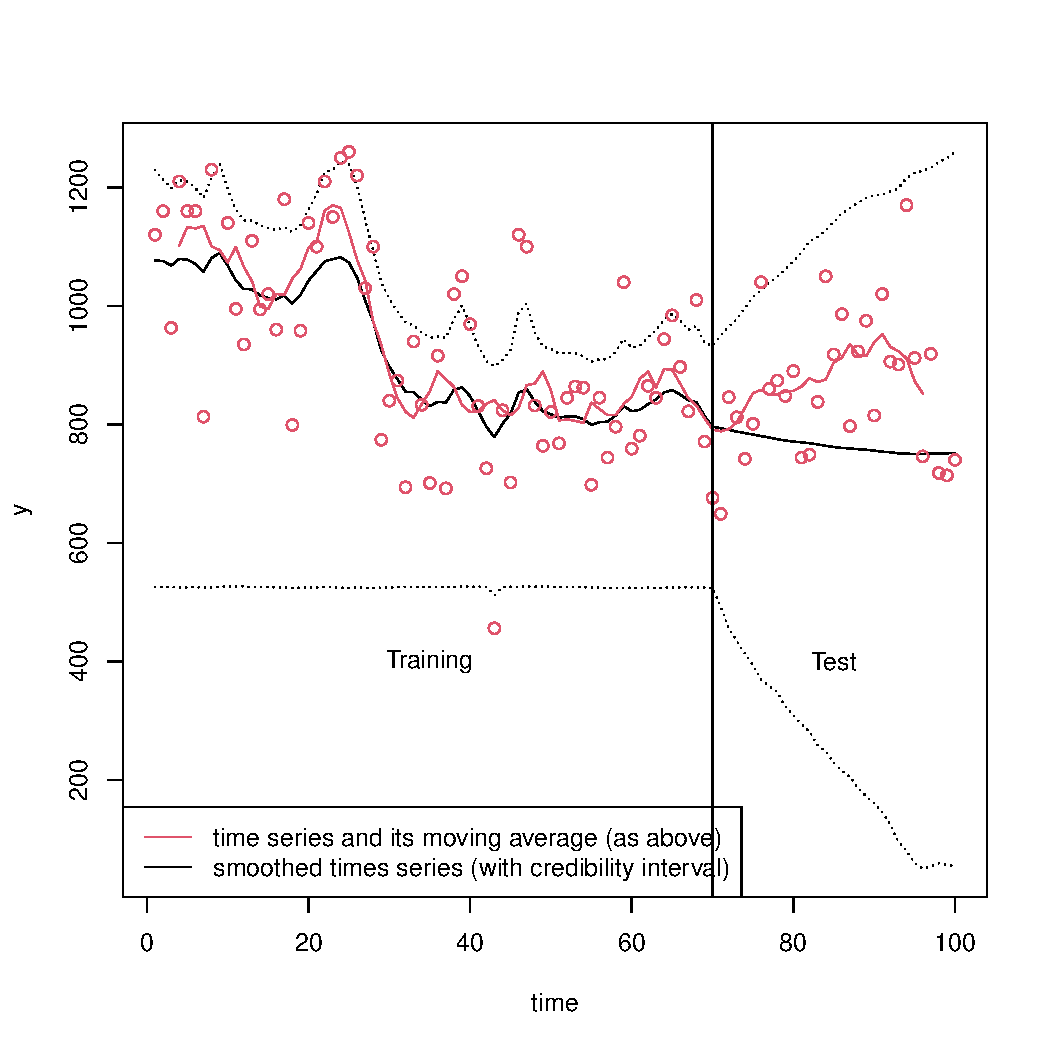
\includegraphics[width=\textwidth]{smoothed_time_series.pdf}
	\caption{Compare smoothed and true time series over time.}
	\label{fig:fig2}
\end{figure}

\begin{figure}
	\centering
	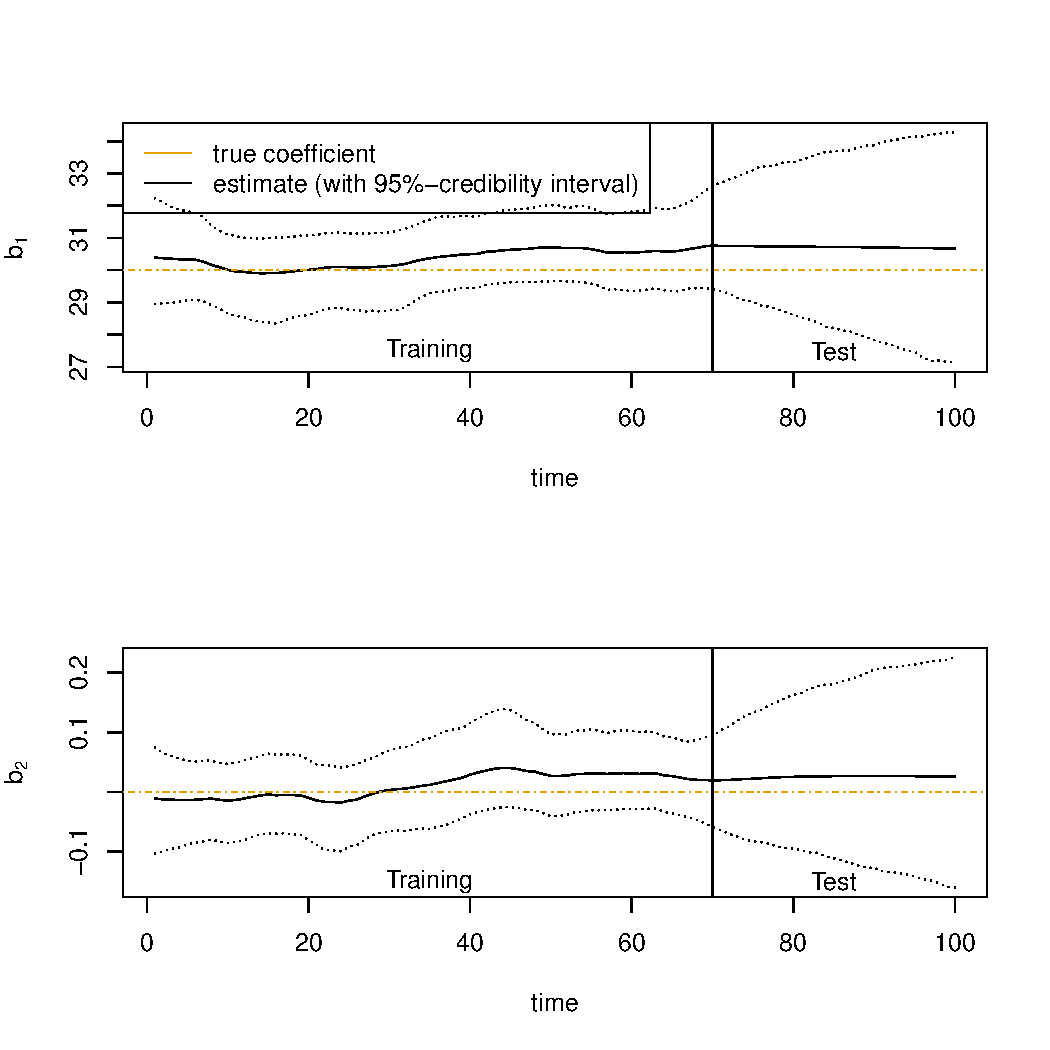
\includegraphics[width=\textwidth]{coefficients_over_time.pdf}
	\caption{Compare estimated and true coefficients $\beta_{1t}$ and $\beta_{2t}$ over time}
	\label{fig:fig3}
\end{figure}

\begin{figure}
	\centering
	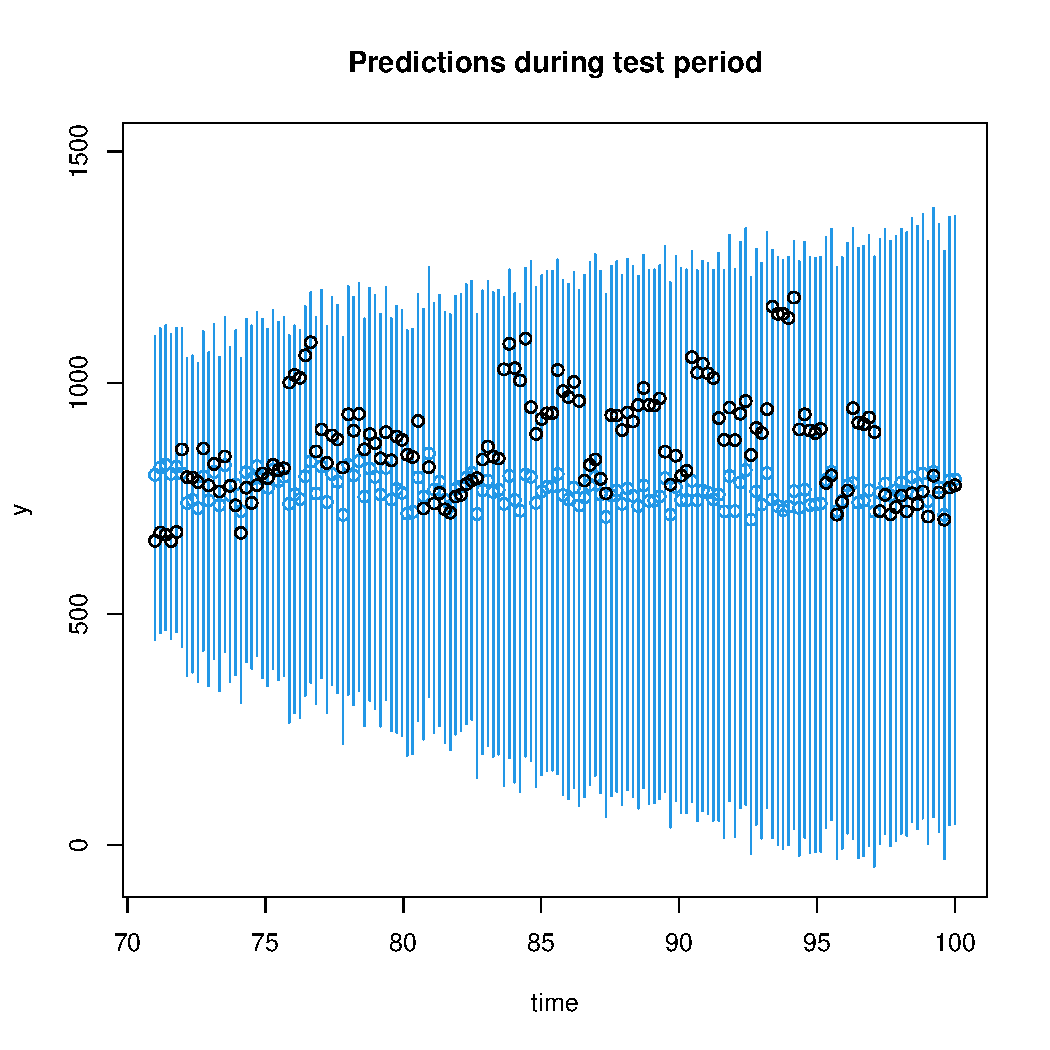
\includegraphics[width=\textwidth]{compare_predictions_with_simulated_data.pdf}
	\caption{Compare predicted values and true values during the test period. Predicted values (with .95-credibility intervals) are shown in blue; True values in black.}
	\label{fig:fig4}
\end{figure}

\section{Simulations for Binary Outcomes}\label{sec:binary}

To model binary outcomes, the observation equation in (1) can easily be changed to a logistic regression,

\begin{eqnarray}
y^{(bin)}_{i(t)} | x_{i(t)p} \sim Bin(1, \textrm{logit}^{-1}(\sum_p x_{i(t)p} \beta_{tp})) & \textrm{(observation equation)}
\end{eqnarray}
without making other changes.

However, meaningful results as shown for continuous outcomes above cannot be replicated with binary outcomes. In three simulations, we 

\begin{enumerate}
    \item draw the outcome $y^{(bin)}_{i(t)}$ from a Bernoulli distribution with probability $p = \textrm{logit}^{-1}(ts_t - 919.35 + 30 \cdot x_{i1} + 0 \cdot x_{i2})$
    \item set $y^{(bin)}_{i(t)}$ to 1 if $y_{i(t)} > ts_t + 30 \cdot x_{i1} + 0 \cdot x_{i2}$
    \item set $y^{(bin)}_{i(t)}$ to 1 if $y_{i(t)} > 900$
\end{enumerate}

For the third simulation, the MCMC-chains do not mix and we are unable to determine the posterior distribution. For the first two simulations, we obtain similar warnings, but preliminary graphical checks indicate that sufficient mixing occurred. Yet, the estimates do not resemble the true values from the simulation in any meaningful way.

The model was also tested with the DonorsChoose dataset, but the MCMC chains did not mix.

\section{Discussion}\label{sec:discussion}

We proposed a new approach for time-related data analysis, applying concepts from the state space literature to model how parameters in least-square regressions change over time. Our simulation provides promising results for continuous outcomes. However, our main goal was to apply this approach with binary outcomes and logistic regression, and this was not successful.

To move forward, we recommend further simulation studies. For binary outcomes, we wonder under which circumstances one could still make progress, or if there are theoretical arguments against it. For continuous outcomes, we argued that our approach should be most fruitful in the presence of long-term trends or sudden shocks, but this reasoning should be confirmed in simulation studies.

Our observation equation, least-squares regression, assumes linearity of parameters, making it rather restrictive. Interactions would need to be hand-coded. Statistical learning algorithms allow the estimation of more flexible functional forms and automated variable selection. This promises better performance and increases efficiency in feature engineering, making statistical learning the preferred option for many. It would be great if future research finds ways to combine statistical learning approaches with state space methodology to improve predictive accuracy while modeling prognostic uncertainty.



\bibliographystyle{unsrtnat}
\bibliography{references2}  %%% Uncomment this line and comment out the ``thebibliography'' section below to use the external .bib file (using bibtex) .


%%% Uncomment this section and comment out the \bibliography{references} line above to use inline references.
% \begin{thebibliography}{1}

% 	\bibitem{kour2014real}
% 	George Kour and Raid Saabne.
% 	\newblock Real-time segmentation of on-line handwritten arabic script.
% 	\newblock In {\em Frontiers in Handwriting Recognition (ICFHR), 2014 14th
% 			International Conference on}, pages 417--422. IEEE, 2014.

% 	\bibitem{kour2014fast}
% 	George Kour and Raid Saabne.
% 	\newblock Fast classification of handwritten on-line arabic characters.
% 	\newblock In {\em Soft Computing and Pattern Recognition (SoCPaR), 2014 6th
% 			International Conference of}, pages 312--318. IEEE, 2014.

% 	\bibitem{hadash2018estimate}
% 	Guy Hadash, Einat Kermany, Boaz Carmeli, Ofer Lavi, George Kour, and Alon
% 	Jacovi.
% 	\newblock Estimate and replace: A novel approach to integrating deep neural
% 	networks with existing applications.
% 	\newblock {\em arXiv preprint arXiv:1804.09028}, 2018.

% \end{thebibliography}


\end{document}
